\documentclass[11pt, a4paper]{article}
\usepackage{ifxetex}
\usepackage{amsmath}
\usepackage[hyperindex,colorlinks,citecolor=cyan,linkcolor=gray,urlcolor=blue
			]{hyperref}

\ifxetex
	\usepackage{fontspec}
	\usepackage{unicode-math}
	\setmainfont[Ligatures=TeX,
		Extension=.otf,
		BoldFont=*-bold,
		UprightFont=*-regular,
		ItalicFont=*-italic,
		BoldItalicFont=*-bolditalic,
	SmallCapsFeatures={Letters=SmallCaps}]{texgyrepagella}
	\setmathfont[Ligatures=TeX]{texgyrepagella-math.otf}
	
	% set up Heros (Helvetica)
	\setsansfont[Ligatures=TeX,
		Extension=.otf,
		BoldFont=*-bold,
		UprightFont=*-regular,
		ItalicFont=*-italic,
		BoldItalicFont=*-bolditalic,
	SmallCapsFeatures={Letters=SmallCaps}]{texgyreheros}
\else
	\usepackage[utf8]{inputenc}
	\usepackage[T1]{fontenc}
\fi

\usepackage{ngerman}
\usepackage{booktabs}
\usepackage{microtype}

\usepackage{svg}
\usepackage{graphicx}
\graphicspath{{../img/}}


\title{Grapheigenschaften auf Kookkurrenzgraphen in Leichter und Standardsprache auf Wikipedia- und Nachrichtencorpora}
\author{Author 1, Author 2, Author 3\\Modul "`Fortgeschrittene Methoden des Information Retrieval"'}
\date{\today}

\begin{document}
\maketitle
\tableofcontents

%%%%%%%%%%%%%%%%%%%%%%%%%%%%%%%%%%%%%%%%%%%%%%%%%%%%%%%%%%%%%%%%%%%%%%%%%%%%%%%%
\section{Motivation und Ziel}

Leichte oder auch Einfache Sprache ist eine Untermenge der deutschen Sprache,
die auf besonders leichte Verst\"andlichkeit optimiert ist. Sie umfasst unter
anderem spezielle Sprachregelungen, typographische Empfehlungen und
Rechtschreibregeln. 

Das \emph{Netzwerk Leichte Sprache} definiert folgende grundlegenden
Eigenschaften Leichter Sprache\cite{nls_regeln} (Auszug):

\begin{enumerate}
	\item Benutzen Sie einfache W\"orter
	\item Benutzen Sie W\"orter, die etwas genau beschreiben
	\item Benutzen Sie bekannte W\"orter und verzichten sie auf Fachw\"orter und Fremdw\"orter
	\item Benutzen Sie immer die gleichen W\"orter f\"ur gleiche Dinge
	\item Benutzen Sie kurze W\"orter
	\item Verzichten Sie auf Abk\"urzungen
	\item Benutzen Sie Verben
	\item Vermeiden Sie den Genitiv und Konjunktiv
	\item Vermeiden Sie Kolloquialismen und bildliche Sprache
	\item Benutzen Sie Ziffern anstatt von Worten
	\item Schreiben Sie kurze S\"atze, die nur eine Aussage enthalten
	\item Benutzen Sie einen einfachen Satzbau
\end{enumerate}

Das englische \"Aquivalent zu Leichter Sprache ist \emph{Simple English}. Es
existieren verschiedene Modelle des Simple English, welche unterschiedliche
Ziele erreichen sollen -- z.B. das \emph{Simplified Technical English}, eine
kontrollierte Sprache f\"ur technische Handb\"ucher. Aufgrund dieser
konkurrierenden Ans\"atze gibt es keine einheitliche Definition oder
Sprachpraxis des Simple English.

% TODO: Was war nochmal Motivation und Ziel?


%%%%%%%%%%%%%%%%%%%%%%%%%%%%%%%%%%%%%%%%%%%%%%%%%%%%%%%%%%%%%%%%%%%%%%%%%%%%%%%%
\section{Werkzeuge}

\subsection{Programmiersprache Python}
Nach sprachunanbhängigen Recherchen über verwendbare Bibliotheken haben wir uns
wegen der bereits implementierten Graphalgorithmen in \texttt{graph-tool} für
die Programmiersprache Python\footnote{\url{https://www.python.org/}}
entschieden.
Wegen der nativen Unicode-Unterstützung wurde Python 3 gewählt.

\subsection{Graphen-Bibliothek \texttt{graph-tool}}
\texttt{graph-tool}\footnote{\url{http://graph-tool.skewed.de/}} ist ein
Python-Modul, welches der Erstellung, Manipulation und statistischen
Auswertung von Graphen dient. Es stellt im Kern einen C++-Wrapper um die Boost
Graph Library dar, wodurch eine \"ahnliche Performanz zu nativen C-Bibliotheken
erreicht wird. Es ist zus\"atzlich in der Lage, Graphen mit modernen Techniken
zu visualisieren und \"ubliche Ma\ss{}e wie Clustering-Koeffizienten, Knoten-
und Kantengrade und Durchmesser zu berechnen.

\subsection{NLP-Framework NLTK}
Das Natural Language Toolkit (NLTK\footnote{\url{http://www.nltk.org/}}) ist
ein Framework f\"ur die Verarbeitung natürlicher Sprache in Python.
Die verwendeten Stopwortlisten für Deutsch und Englisch stammen aus der
Bibliothek nltk-data.


%%%%%%%%%%%%%%%%%%%%%%%%%%%%%%%%%%%%%%%%%%%%%%%%%%%%%%%%%%%%%%%%%%%%%%%%%%%%%%%%
\section{Datenbasis}

Als Datenbasis wurden Quellen gew\"ahlt, die sich durch eine gro\ss{}e
semantische und logische N\"ahe auszeichnen, namentlich Nachrichtenseiten in
deutscher und Wikipediaartikel in englischer Sprache.

\subsection{Nachrichtenseiten}
\label{nrseiten}

\subsubsection{nachrichtenleicht.de (nl)}

Nachrichtenleicht ist ein Dienst des Deutschlandfunks, welcher einmal
w\"ochentlich die wichtigsten Nachrichten der vorangegangenen Woche in Leichter
Sprache zusammenfasst. Er soll die mehreren Millionen Menschen in Deutschland
erreichen, die aus verschiedenen Gr\"unden von konventionellen
Nachrichtenangeboten ausgeschlossen sind.

\subsubsection{deunews2010\_10K Corpus der ASV (denews10k)}

Als korrespondierende Datenquelle in Standardsprache wurde der
deunews\-2010\_10K-Corpus des Lehrstuhls f\"ur automatische Sprachverarbeitung
(ASV) der Universit\"at Leipzig gew\"ahlt. Dieser weist eine \"ahnliche Satzzahl
zu den von nachrichtenleicht extrahierten Text auf und wurde bereits von der ASV
normalisiert \cite{Quasthoff2006}.

\subsection{Wikipedia (wiki\_sim bzw. wiki\_en)}
\label{corp-wiki}
Die zweite Datenquelle sind Artikel aus der Wikipedia in \emph{Simple} und
\emph{Standard English}. Mit fast 120.000 Lemmata stellt die Simple English
Wikipedia eine der gr\"o\ss{}ten \"offentlich frei verf\"ugbaren Textsammlungen
in einer Leichten Sprachvariante dar.
Zus\"atzlich ist ein Dokumentenalignment zwischen den zwei Sprachvarianten
vorhanden, was die einfache Erstellung zweier inhaltlich homogener Corpora
gestattet.


%%%%%%%%%%%%%%%%%%%%%%%%%%%%%%%%%%%%%%%%%%%%%%%%%%%%%%%%%%%%%%%%%%%%%%%%%%%%%%%%
\section{Vorverarbeitung}

\subsection{Datenextraktion und Erstellung der Corpora}
\label{datextr}

Mittels eines selbstgeschriebenen Crawlers wurden die relevanten Textmengen
heruntergeladen, extrahiert und zu Corpora zusammengefasst.

Nachrichtenleicht wurde rekursiv von der Startseite aus gequeriet
und die resultierenden Texte in einer MongoDB gespeichert.
Dabei wurden Überschriften, Teaser und Nachrichtentexte jeweils seperat erfasst
und schließlich Teaser und Nachrichteninhalt zum Corpus hinzugefügt.

Zur Erstellung der Wikipedia-Corpora wurde zunächst eine Liste aller
in Simple English verfügbaren Artikel erstellt. Anschließend wurden diese
zusammen mit dem jeweils korrespondierenden Artikel in Standard English
heruntergeladen und im Rohformat (mit eingebettetem MediaWiki-Markup) in einer
JSON-Datei gespeichert.

Die Entfernung des Mediawiki-Markups und die Überführung in Reintext stellte
sich dabei als eine nichttriviale Aufgabe dar.
Mit dem MediaWiki Parser from
Hell\footnote{\url{http://mwparserfromhell.rtfd.org}} existiert ein vollständiger
Parser für Mediawiki-Markup.
Für die entsprechende Datenmenge (ca. 2~GB Rohdaten) erwies sich dieser jedoch
als deutlich zu langsam und somit für die Bereinigung ungeeignet.
\\
Abhilfe schuf ein selbst entwickeltes Python-Skript, welches Markup mit Hilfe
regul\"arer Ausdr\"ucke und rekursiver Funktionsaufrufe entfernt bzw. umwandelt.
Dies gestattete zufrieden stellende Ergebnisse mit vertretbarem Zeitaufwand.

Nach Entfernen des Wiki-Markups wurden die Artikel auf die Satzanzahl
des jweils k\"urzeren Artikels reduziert und anschliessend in einer MongoDB
gespeichert.


\subsection{Berechnung der Kookkurrenzen}

Die Kookkurrenzen wurden von mittels der Pipeline des Lehrsstuhls f\"ur
Automatische Sprachverarbeitung für uns berechnet (siehe \cite{Quasthoff2006})
und in eine MySQL-Datenbank eingepflegt.


\subsection{Erstellung der Graphen}

Die errechneten Kookkurrenz-Paare wurden zunächst gefiltert. Dabei wurden 
\begin{itemize}
    \item Lemmata, welche Leerzeichen, Kommata oder andere Satzzeichen enthalten
    \item Lemmata der Zeichenlänge 1
    \item Kookkurrenzen zwischen zwei identischen Lemmata
\end{itemize}
entfernt, so dass schließlich nur Kookkurrenzen zwischen einzelnen Wörtern
zurückblieben.
Außerdem wurden -- da wir mit einem ungerichteten Graphen arbeiten -- identische
Kookkurrenzpaare entfernt, so dass am Ende jedes Paar nur einmal auftrat.

Die verbleibenden Kookkurrenzpaare wurden in \texttt{graph-tool}-Objekte geparst
und zu einem corpusumfassenden Kokkurrenzgraphen zusammengesetzt.

Um sinnvolle Berechnungen von Weglängen etc. anzustellen, erwies es sich als
notwendig, den so erzeugten Graphen auf die größte Zusammenhangskomponente zu
reduzieren und nicht verbundene Subgraphen zu verwerfen.
Die Kanten- und Knotenanzahl vor und nach diesem Schritt sind Tabelle
\ref{tab-zsf} zu entnehmen.

Anschließend wurden die relevanten Berechnungen (vgl. Abschnitt
\ref{berechnung-ergebnisse}) durchgeführt und Ergebnisse ausgegeben.
Auch die Daten zur Erstellung der Histogramme wurden in diesem Schritt
gespeichert, um sie anschließend nach R zu importieren und dort mittels ggplot2
grafisch aufzubereiten.

Um Kookkurrenzgraphen für einzelne Wörter auszugeben, wurden Subgraphen aus dem
Corpusgraphen wurden mittels eines \texttt{force-directed graph} nach
\cite{Hu2006} gelayoutet.


%%%%%%%%%%%%%%%%%%%%%%%%%%%%%%%%%%%%%%%%%%%%%%%%%%%%%%%%%%%%%%%%%%%%%%%%%%%%%%%%
\section{Berechnung der Graphenkenngr\"o\ss{}en und Ergebnisse}
\label{berechnung-ergebnisse}

Nach Erstellung der Graphen sollen diese auf typische Kenngrößen untersucht,
anhand dieser charakterisiert sowie paarweise verglichen werden (deutsch vs.
englisch, Leichte vs. Standardsprache).
Für verschiedene Eigenschaften bietet \texttt{graph-tool} bereits implementierte
Algorithmen an. Im Folgenden werden die Kenngrößen kurz erläutert, unsere
Erwartungen dargestellt und die Ergebnisse gezeigt.

\subsection{Gr\"o\ss{}e (Knotenzahl)}
\label{groesse-knotenzahl}

Schon in der Größe der Graphen sollten sich paarweise Unterschiede erkennen
lassen. So sollten die beiden Corpora in Leichter Sprache wesentlich weniger
verschiedene Wörter enthalten. Durch die Praxis, schwierige Wörter
durch leichter verständliche zu ersetzen, ist zu erwarten, dass erstere im
Leichten Corpus nicht vorkommen. Die Anzahl der Knoten lässt sich trivial
auszählen.

Der deunews2010\_10K-Corpus hat 3205 Knoten, wovon 3142 auf die größte
Zusammenhangkomponente entfallen.
Nachrichtenleicht weist mit 2946 (resp. 2766) im Vergleich eine etwas geringere
Knotenzahl auf.
Die Wikipedia-Corpora enthielten mehr Text und somit sind auch die Graphen
deutlich größer: 45897 (45446) Knoten entfallen auf die englische, 36582 (36131)
auf die \emph{simple english} Variante.

Es l\"asst sich also schlie\ss{}en, dass diese grundlegende Erwartung,
leichte Sprache enthielte bei gleicher Satzzahl weniger unterschiedliche Wörter,
erf\"ullt ist.

\subsection{Rang der Knotengrade}

Wie in Abb. \ref{fig-vdeg} dargestellt, folgt die Verteilung der Knotengrade
dem Zipfschen Gesetz.

\begin{figure}[ht]
    \centering
        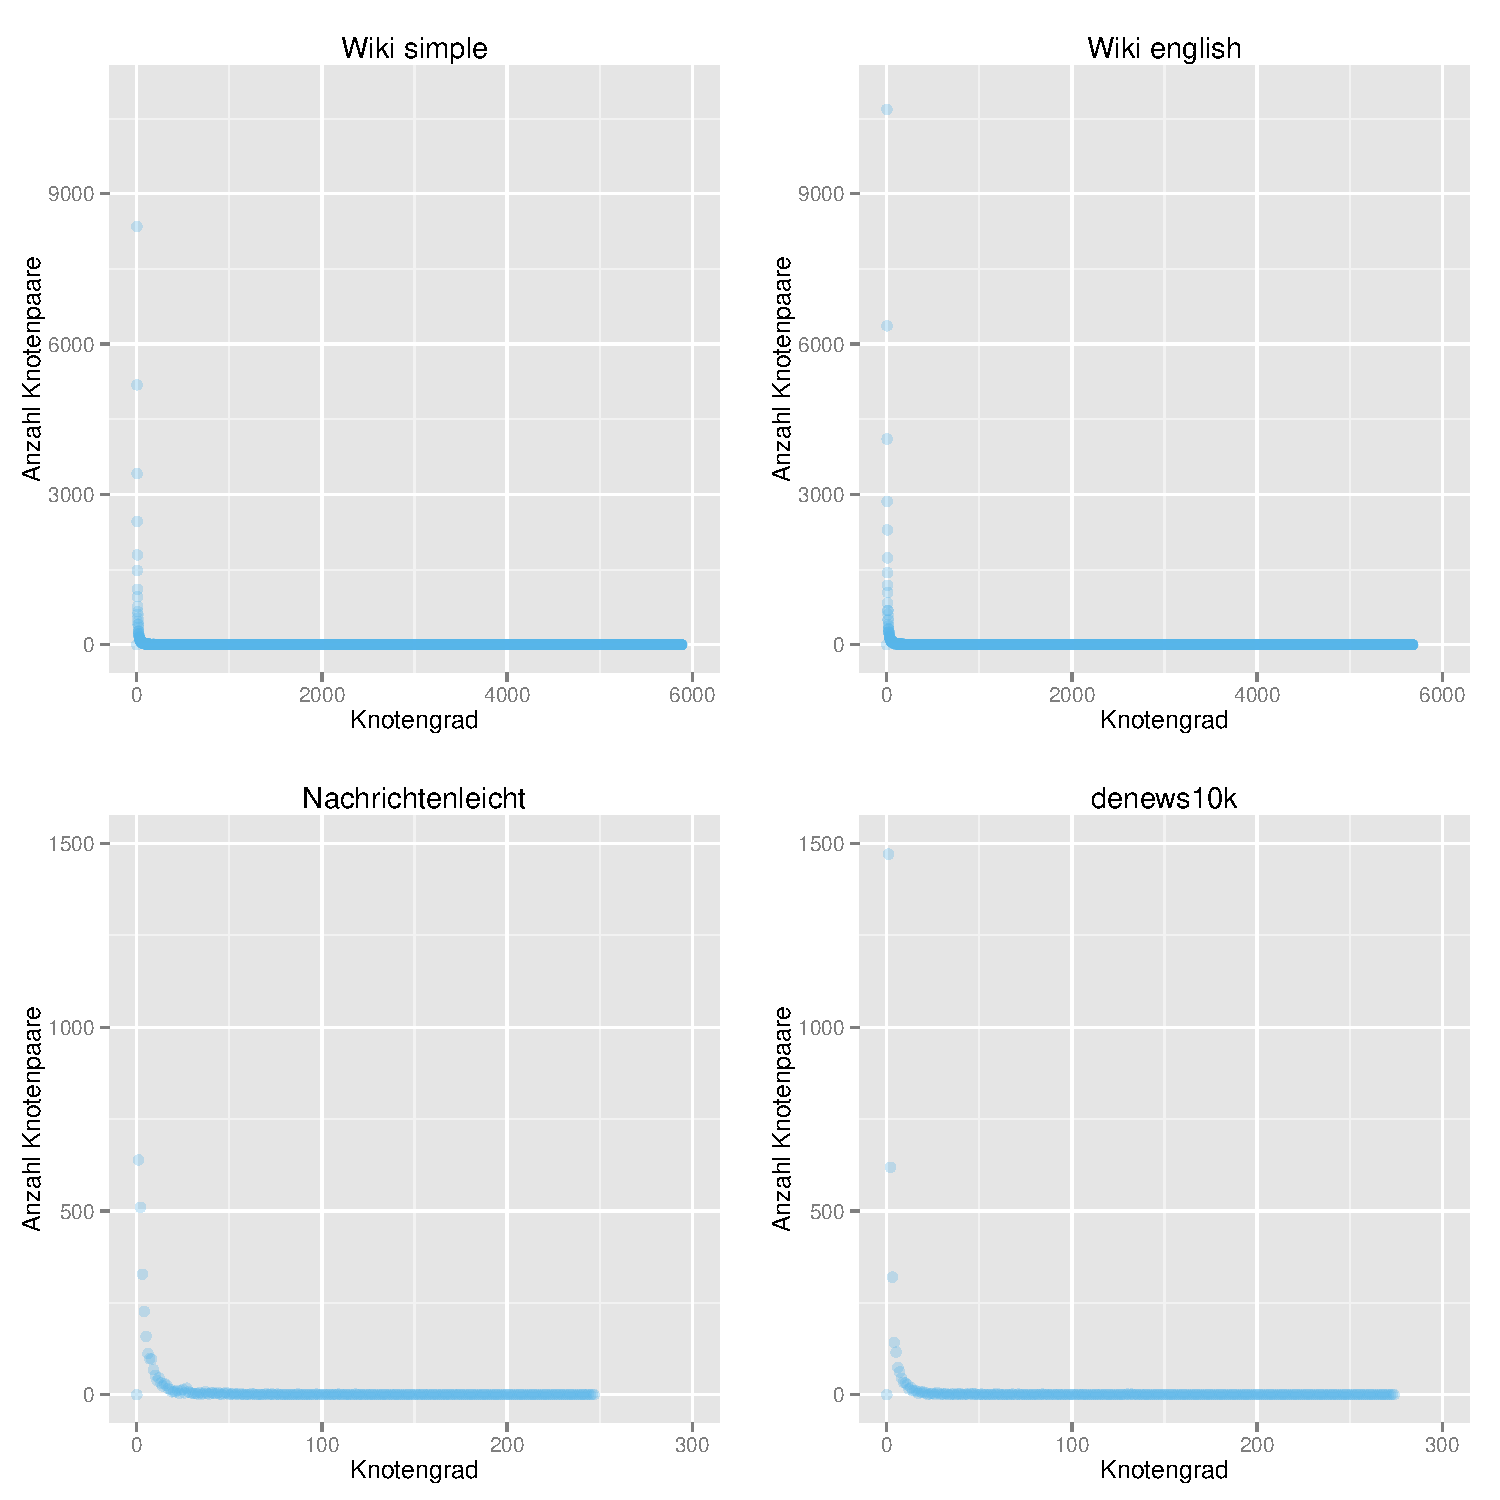
\includegraphics[scale=.5]{vdeg_plots.pdf}
    \caption{Verteilung der Knotengrade nach Corpus}
    \label{fig-vdeg}
\end{figure}


\subsection{Dichte}

Die Dichte eines Graphen beschreibt das Verhältnis von vorhandenen Kanten zu
potentiell möglichen Kanten.
Ein Wert von $1$ bedeutet, dass jeder Knoten mit jedem anderen Verbunden ist
(vollständiger Graph), dem gegenüber eine $0$, dass keine Kanten vorhanden sind.
Die Dichte wird wie folgt berechnet:

$$
    \frac{|E|}{|V|\left(|V|-1\right)}
$$

$|E|$ ist die Anzahl der Kanten, $|V|$ die Anzahl der Knoten im Graphen. 

Für die einfachen Sprachvarianten sollten unseren Erwartungen zufolge die
Graphen dichter sein als für Standardsprache.
Wie bereits beschrieben, gibt es in ersteren weniger Vokabular, dementsprechend
weniger Knoten, die potentiell verbunden werden können. Die Vorhandenen kommen
jedoch öfter gemeinsam vor und sind somit enger verknüpft.

\begin{table}[ht]
  \centering
  \begin{tabular}{ll}
    \toprule
    Corpus            &         Dichte (in $10^{-4}$)\\
    \midrule
    nl                &  		15,090239 \\
    denews10k         &  		7,737342 \\
    wiki\_sim         &  		2,844456 \\
    wiki\_en          &  		2,489951 \\
    \bottomrule
  \end{tabular}
  \caption{\label{density_table} Graphdichte nach Corpus}
\end{table}

Die Ergebnisse in Tabelle \ref{density_table} bestätigen diese Vermutung.
Insgesamt haben alle Graphen eine Dichte von $<0,01$, was für
Kookkurrenzgraphen in einem erwartbaren Rahmen liegt.

Der nachrichtenleicht-Corpus weist mit $15,1\cdot 10^{-4}$ eine fast doppelt so
hohe Dichte auf wie denews10k ($7,74\cdot 10^{-4}$).\\
Bei den englischen Corpora fällt der Unterschied etwas geringer aus.
Dennoch weist die reguläre Sprachvariante auch hier eine ca. 14\% geringere
Dichte auf als die Leichte Sprache.

Dass die Graphen der Wikipedia-Corpora eine geringere Dichte haben, lässt sich
mit der in einer Enzyklopädie zu erwartenden höheren Themenvielfalt gegenüber
den Nachrichteninhalten erklären.
Dies bedeutet mehr potentiell auftretende unterschiedliche Wörter, die jedoch
nicht alle in den gleichen Kontexten auftreten und somit nur in begrenztem
Umfang Kanten zum Graphen hinzufügen, der Quadratische Zusammenhang der Dichte
führt somit zu deutlich niedrigeren Werten. 

\subsection{Small-World-Eigenschaften}
Small-World-Graphen zeichnen sich durch kleine Durchmesser und hohe Clusterkoeffizienten aus. Diese Werte sind im Vergleich zu Zufallsgraphen zu betrachten. Dementsprechend gibt es Messwerte, die genau diese Relation versuchen in einem Wert zusammenzufassen um damit eine Aussage über Small-World-Eigenschaften zu machen. 

\subsubsection{Clusterkoeffizient}

Eng mit der Dichte verwandt ist der Clusterkoeffizient. Er beschreibt die
Anzahl vorhandener Dreiecke im Graph im Verhältnis zu möglichen Dreiecken. Drei
Knoten, die jeweils paarweise verbunden sind, bilden ein Dreieck. Ziel ist ein
Messwert, der aussagt, wie sehr die Knoten Cliquen bilden. Lokal betrachtet
bedeutet der Wert die Wahrscheinlichkeit, die Nachbarn eines Nachbarn zu kennen.
Dies lässt sich realweltlicht sehr anschaulich beschreiben: Kennt ein Mensch die 
Freunde seiner Freunde?
Da wir die Graphen global miteinander vergleichen möchten, verwenden wir den
globalen Clusterkoeffizienten $C$. Er berechnet sich wie folgt:

$$
    C = \frac{3\cdot\text{Anzahl der Dreiecke}}{\text{Anzahl verbundener Tripel}}
$$

Ein Tripel bezeichnet drei miteinander verbundene Knoten, nicht
notwendigerweise ein Dreieck. Knoten A kann mit Knoten B und C verbunden sein,
während B nicht mit C verbunden ist.

In \emph{Small-World-Graphen} ist der Clusterkoeffizient typischerweise hoch, 
insbesondere verglichen mit Zufallsgraphen gleicher Größe, also gleicher Anzahl
Knoten und Kanten\cite{Newman2003}.\\


\subsubsection{Durchmesser und minimale Wegl\"angen}
Um Small-World-Eigenschaften nachzuweisen, ist es außerdem interessant, die
Weglängen im Graphen zu untersuchen. Eine gute Kenngröße ist dabei der Durchmesser
des Graphen, also der längste minimale Weg zwischen zwei Knoten. In einer
\emph{small world} sind alle Knoten von allen anderen in wenigen Schritten
erreichbar, typischerweise in etwa 6 Schritten, die sogenannten 
\emph{six degrees of separation}(siehe beispielsweise \cite{Newman2003}). 
\texttt{graph-tool} erlaubt zum einen die Ausgabe eines Durchmessers, wie oben
 beschrieben, und zum anderen die Ausgabe eines Histogramms, welches die 
Häufigkeit der Längen aller kürzesten Wege darstellt (siehe Abb. \ref{fig-mdh}).

% latex table generated in R 3.2.0 by xtable 1.7-4 package
% Mon Apr 20 13:50:42 2015
\begin{table}[ht]
    \centering
    \begin{tabular}{rrrrr}
      \toprule
    Weglänge       & nl          & denews10k   & wiki\_sim   & wiki\_en     \\ 
      \midrule
      1            & 0,30        & 0,15        & 0,06        & 0,05         \\ 
      2            & 10,66       & 6,69        & 14,94       & 12,95        \\ 
      3            & 49,35       & 46,26       & 63,60       & 64,48        \\ 
      4            & 34,55       & 41,83       & 20,25       & 21,30        \\ 
      5            & 4,61        & 4,70        & 1,11        & 1,17         \\ 
      6            & 0,47        & 0,35        & 0,04        & 0,04         \\ 
      7            & 0,07        & 0,01        & $\sim$0,00  & $\sim$0,00   \\ 
      8            & $\sim$0,00  & $\sim$0,00  & $\sim$0,00  & $\sim$0,00   \\ 
      9            & $\sim$0,00  & 0           & 0           & 0            \\ 
      Summe        & 100,00      & 100,00      & 100,00      & 100,00       \\ 
      Durchschnitt & 3,34        & 3,45        & 3,08        & 3,11         \\
       \bottomrule
    \end{tabular}
    \caption{Anteil der Weglängen paarweiser kürzester Wege zwischen allen Knoten, in Prozent}
    \label{md-perc}
\end{table}

\begin{figure}[ht]
    \centering
        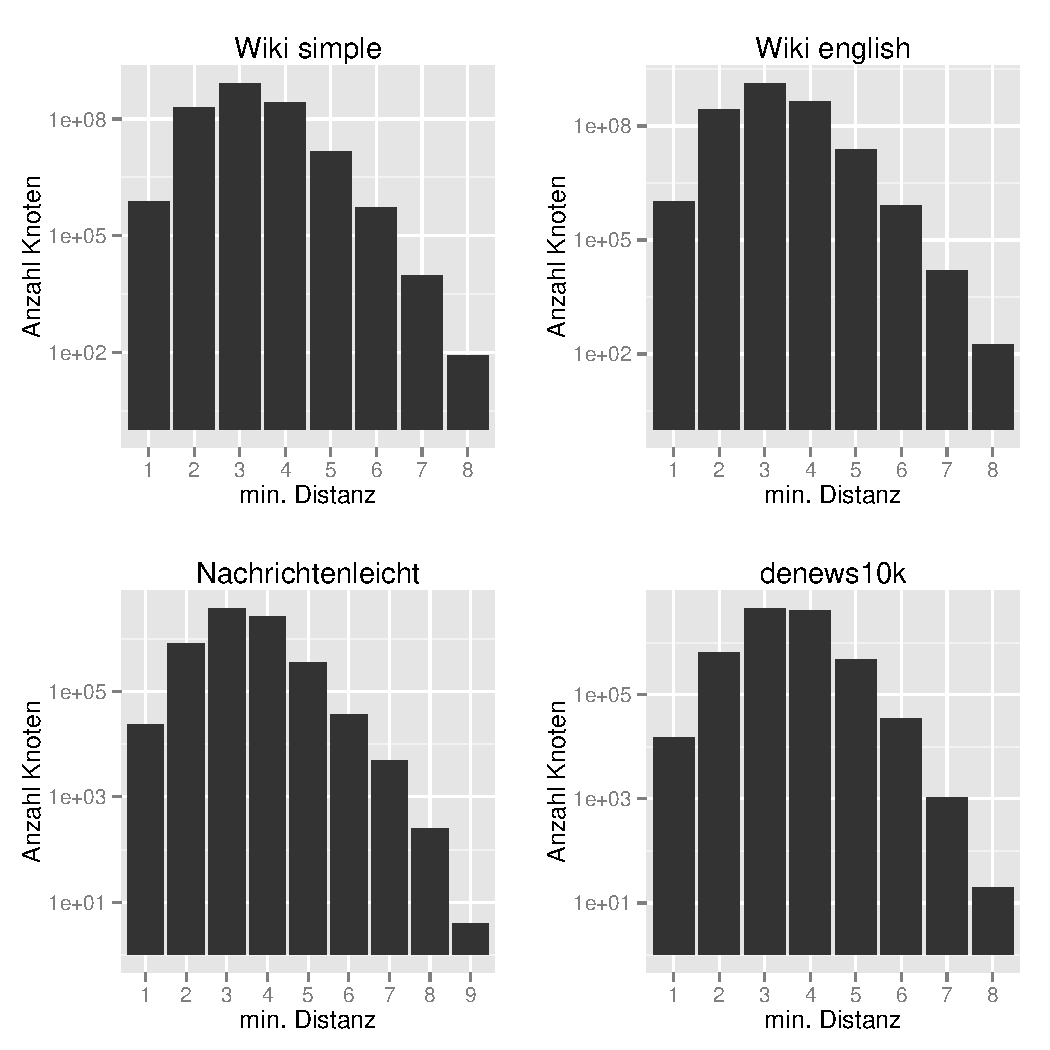
\includegraphics[scale=.75]{mdh_plots.pdf}
    \caption{Verteilung der minimalen Weglängen nach Corpus}
    \label{fig-mdh}
\end{figure}

\subsubsection{Small-World-Messwert}
Humphries et al. benennen in \cite{Humphries2006} einen Messwert vor der deutlich
machen soll, ob ein Graph ein Small-World-Graph ist oder nicht. Sie setzen hierzu
die Weglängen und die globalen Clusterkoeffizienten von Graphen in Relation. 
Dabei sind Clusterkoeffizienten insbesondere in gitterartigen Netzwerken hoch und
kurze Weglängen zeichnen besonders Zufallsgraphen aus. Um diese Erkentnisse zu
verbinden werden die beiden Messwerte des zu testenden Graphen mit denen eines
vergleichbaren Zufallsgraphen relativiert. Der Zufallsgraph wird aus dem 
Ursprünglichen durch zufallsbasiertes \emph{rewiring} gewonnen, es soll dabei die
Verteilung der Knotengrade beibehalten werden. Die Kanten werden gleichverteilt
neu verbunden, jede zu erstellende Verbindung hat die gleiche Wahrscheinlichkeit.
Die Bibliothek \texttt{graph\_tool} stellt dazu den notwendigen Algorithmus zur 
Verfügung\footnote{\url{http://graph-tool.skewed.de/static/doc/generation.html\#graph_tool.generation.random_rewire}},
der eben die Knotengradverteilung beibehält.\\
Das vorgeschlagene Maß setzt sich wie folgt zusammen:

$$
\sigma = \frac{C/C_{rand}}{ L/L_{rand}}
$$

Wobei $L$ der durchschnittliche kürzeste Abstand zwischen den Knoten ist und $C$
der Clusterkoeffizient. Wichtigstes Kennzeichen für einen Small-World-Graphen
ist hier dass $C \gg C_{rand}$, während $L \approx L_{rand}$, sodass $\sigma > 1$.\\


\subsubsection{Ergebnisse}
\paragraph{Clusteringkoeffizient}
In Tabelle \ref{tab-zsf} sind die Ergebnisse der vorgestellten Maße aufgelistet, darunter die Clusteringkoeffizienten der Graphen. Paarweise bezüglich Corpussprache verglichen zeigt sich, dass die beiden englischen Corpora sehr ähnliche Koeffizienten aufweisen, beide knapp über $0,04$. Größer ist der Unterschied zwischen den beiden deutschen Sammlungen, in leichter Sprache ergibt sich ein Wert von etwa $0,06$, wogegen dieser bei normaler Sprache lediglich $0,03$ beträgt. Die leichte Sprache ist hier also deutlich stärker geclustert. Jedoch verglichen mit Graphen aus \cite[S. 182]{Newman2003} sind die Werte alle sehr klein. Insbesondere der Vergleich zu Zufallsgraphen gleicher Größe ist interessant, die Tabelle liefert auch dafür die Ergebnisse: Der Quotient aus $C/C_{rand}$ ist in allen Fällen unter $1$, für \texttt{nachrichtenleicht} liegt er bei $0,96$, der ursprüngliche Graph und sein Zufällig verändertes Pendant haben also beinahe den selben Clusteringkoeffizienten. Zusammengefasst ist deutlich erkennbar, dass die Clusteringkoeffizienten nicht in Wertebereichen liegen, die für Small-World-Eigenschaften notwendig wären.

\paragraph{Durchmesser und Weglängen}
Für die Graphdurchmesser zeigen sich jedoch andere Ergebnisse. Typischerweise lassen sich alle Knoten innerhalb von etwa 6 Schritten von jedem anderen Knoten erreichen. Tabelle \ref{md-perc} bestätigt diese These. Es sind nur wenige Wortpaare ausserhalb dieser Grenze, diese werden im nächsten Abschnitt und Kapitel \ref{sec:aussen_liegende} mit Hilfe von Visualisierungen detailiert betrachtet. Es zeigt sich bei allen Graphen, dass die Ränder dieser aus selten verwendeten Namen bestehen.
Die Tabelle zeigt sehr deutlich, dass die meisten Paare innerhalb von 3-4 Schritten verbunden sind, es gibt kaum Pfade, die länger sind. Die Durchschnittswerte liegen bei allen vier Graphen knapp über 3. Für Small-World-Graphen wäre ein etwas höherer Durchschnitt typischer gewesen(vgl \cite{Newman2003}), die sich bei sozialen Netzwerken um $5$-$7$ bewegen (für den dort ebenfalls erwähnten Wortkookkurrenzgraphen ist kein Wert angegeben).   

\paragraph{Aussen liegende Wörter}
Wie beschrieben machen Namen den äußeren Rand der Graphen aus, so sind etwa \emph{Seymour} und \emph{Hoffman} im \texttt{nachrichtenleicht}-Corpus lediglich ein mal vorgekommen, im Zuge der Todesnachricht des Schauspielers. Des öfteren ist zu beobachten, dass Fremdsprachige Namen die Graphgrenzen ausmachen, so liegen im englischsprachigen \texttt{wiki-sim}-Corpus \emph{Che Guevara}, \emph{Kamui Kobayashi}, \emph{Kazimir Malevich} und die \emph{Frankfurter Allgemeine Zeitung} ganz aussen. Bei \texttt{denews10k} sind \emph{Microsoft}, \emph{Windows}, und \emph{Phone} in Zusammenhang aussen, oder auch \emph{Financial} und \emph{Times}, jedoch auch \emph{Christoph Metzelder} oder \emph{St. Pauli} und \emph{Christoph Metzelder}. Bei größen von 10.000 Sätzen ist es bei den Nachrichtencorpora nicht verwunderlich, dass aufgrund der Unterschiedlichkeit von behandelten Themen selten genannte Personen am Rand des Graphen erscheinen. Da die Nachrichten auch in sehr begrenzten Zeiträumen gesammelt wurden verstärkt sich dieser Effekt. Das gleiche Problem ergibt sich bei den Wikipediaartikeln, welche unabhängig voneinander gesammelt wurden, es ergibt sich also nicht eine Zusammenhangskomponente an Artikeln sondern aus allen verschiedenen Themengebieten.\\
Namen von Personen, die mehr im Fokus der Öffentlichkeit stehen, etwa \emph{Angela}, \emph{Merkel}, \emph{Obama}, sind verglichen zu den oben genannten deutlich stärker im Graph verbunden. Auch die dort verbundenen Wörter sind Schlüssel dafür, ob ein Wort am Rand oder im Graphen liegt, Verben wie \emph{sagt} verbinden sehr schnell zum Zentrum.

\paragraph{Small-World-Messwert}
Wie die Ergebnisse der Clusteringkoeffizienten bereits andeuten lassen sich mit dem verwendeten Maß nicht nachweisen, dass es sich um Small-World-Graphen handelt. Die Zwischenrechnungen und Ergebnisse sind in \ref{tab-zsf} zu sehen. Zwar sind die durchschnittlichen Weglängen bei den Zufallsgraphen beinahe identisch zu denen der Ursprungsgraphen, jedoch bilden die Wortcorpora nicht genügend Cluster um die Anforderungen zu erfüllen. $C/C_{rand}$ liegt teilweise derart nah beieinander, dass den Graphen lediglich Ähnlichkeit zu Zufallsgraphen nachweisbar ist. Bei denews10k liegt er sogar unter $0,5$, was auch von der geringen Dichte her rührt.

TODO tabelle vielleicht nicht in eigene section, reicht als objekt im irgendwo :)

\subsection{Übersicht der berechneten Größen}
\begin{table}[ht]
    \begin{tabular}{l*{4}{r}}
    \toprule
    Kenngröße                     & nl        & denews10k & wiki\_sim & wiki\_en \\
    \midrule
    $|V|$                         & 2946      & 3205      & 36582     & 45897  \\
    $|E|$                         & 11639     & 7669      & 371559    & 514489 \\
    $|V|$\footnotemark[6]         & 2766      & 3142      & 36131     & 45446  \\
    $|E|$\footnotemark[6]         & 11541     & 7636      & 371319    & 514248 \\
    Dichte (in $10^{-4}$)          & 15,090239 & 7,737342  & 2,844456  & 2,489951 \\
    Clusterkoeffizient            & 0,064516  & 0,033906  & 0,040403  & 0,042299 \\
    CK stdev ($10^{-2}$)           & 0,626338  & 0,470389  & 0,612476  & 0,481688 \\
    $\sigma$                      & 0,970016  & 0,451959  & 0,857932  &         \\
    $C / C_{rand}$                 & 0,961374  & 0,474512  & 0,832651  &         \\
    $L / L_{rand}$                 & 0,991090  & 1,049900  & 0,970532  &         \\
    \dots                         &           &           &           &          \\
    \bottomrule
    \end{tabular}
    \caption{Übersichtstabelle Graphenkenngrößen}
    \label{tab-zsf}
\end{table}
% TODO: nach dem Endlayout sicherstellen, dass die folgene Fußnote an der richtigen
% Stelle auftaucht!
\footnotetext[6]{größte Zusammenhangskomponente}

In Tabelle \ref{tab-zsf} befindet sich eine Zusammenfassung der für die
jeweiligen Corpora berechneten Kenngrößen.


\subsection{H\"aufige W\"orter}

\subsubsection{Nachrichten-Corpora}

\begin{table}[ht]
    \begin{tabular}{l*{2}{lr}}
    \toprule
    Nr. & nl & Häufigkeit & denews10k & Häufikeit\\
    \midrule
    1  & Menschen    & 87 &  Prozent     & 48 \\
    2  & gewonnen    & 69 &  Euro        & 47 \\
    3  & Mannschaft  & 62 &  sagte       & 24 \\
    4  & Geld        & 54 &  Uhr         & 23 \\
    5  & Stadt       & 51 &  Jahren      & 23 \\
    6  & mehr        & 50 &  sei         & 18 \\
    7  & Partei      & 45 &  wurde       & 18 \\
    8  & Land        & 45 &  einfach     & 17 \\
    9  & Dortmund    & 45 &  Artikel     & 16 \\
    10 & Politiker   & 43 &  \textbf{Jahr}        & 16 \\
    11 & Spiel       & 41 &  Dollar      & 15 \\
    12 & bekommen    & 41 &  verwenden   & 15 \\
    13 & \textbf{Jahr}        & 40 &  unten       & 15 \\
    14 & viele       & 38 &  Jahre       & 15 \\
    15 & Bayern      & 36 &  stehenden   & 15 \\
    16 & Preis       & 34 &  Link        & 14 \\
    17 & München     & 34 &  möchten     & 14 \\
    18 & Verein      & 33 &  verlinken   & 14 \\
    19 & deutsche    & 33 &  kostenfrei  & 14 \\
    20 & Film        & 32 &  seit        & 14 \\
    21 & zusammen    & 32 &  dpa         & 14 \\
    22 &             &    &  Millionen   & 14 \\
    \bottomrule
    \end{tabular}
    \caption{Häufigste Worte in den Nachrichten-Corpora}
    \label{words-nachrichten}
\end{table}

Wie in Tabelle \ref{words-nachrichten} zu erkennen, gibt es nur wenige
Überschneidungen des Vokabulars des nachrichtenleicht-Corpus mit denews10k.
Fett gedruckt sind in den Tabellen diejenigen Worte, die in beiden Corpora
vorkommen.
Bei den Nachrichten-Corpora handelt es sich lediglich um das Wort "`Jahr"'.
Dies deutet bereits auf eine gewisse thematische Inhomogenität der Corpora hin.
Dieses Ergebnis ist insofern nicht überraschend, dass die Corpora aus
unterschiedlichen Quellen stammen (vgl. Abschnitt \ref{nrseiten}) und
im Gegensatz zu den Wikipedia-Daten nicht aligniert wurden.
Auch wurden die Ursprungstexte für unterschiedliche Zielgruppen verfasst.

Darüber hinaus zeigt sich, dass Worte im nachrichtenleicht-Corpus generell
häufiger auftreten (häufigstes Wort: Menschen, 87mal; denews: Prozent, 48mal).
Dies bestätigt die Vermutung aus Abschnitt \ref{groesse-knotenzahl}.

Weiterhin wird ersichtlich, dass der nachrichtenleicht-Corpus seinen
thematischen Schwerpunkt auf Politik und Sport legt.
Erkennbar ist dies am häufigen Auftreten der Worte wie Stadt, Partei, Land,
Politiker bzw. Mannschaft, Spiel, Bayern, München, Verein.
Im denews-Corpus treten hingegen häufiger wirtschaftsbezogene Wörter wie Prozent,
Euro, Dollar oder Millionen auf.


\subsubsection{Wikipedia-Corpora}

\begin{table}[ht]
    \begin{tabular}{l*{2}{lr}}
    \toprule
    Nr. & wiki\_sim & Häufigkeit & wiki\_en & Häufikeit\\
    \midrule
     1 & \textbf{born}       & 71 & \textbf{born}         & 86\\
     2 & \textbf{American}   & 52 & \textbf{American}     & 58\\
     3 & \textbf{commune}    & 49 & \textbf{commune}      & 52\\
     4 & \textbf{France}     & 47 & \textbf{France}       & 50\\
     5 & \textbf{won}        & 41 & \textbf{department}   & 49\\
     6 & \textbf{department} & 41 & film                  & 46\\
     7 & movie               & 36 & \textbf{television}   & 43\\
     8 & \textbf{television} & 35 & \textbf{won}          & 42\\
     9 & died                & 33 & \textbf{League}       & 40\\
    10 & people              & 33 & \textbf{County}       & 40\\
    11 & NHL                 & 31 & \textbf{Award}        & 39\\
    12 & actor               & 31 & University            & 39\\
    13 & \textbf{World}      & 30 & series                & 38\\
    14 & United              & 29 & \textbf{released}     & 38\\
    15 & \textbf{League}     & 28 & album                 & 38\\
    16 & National            & 28 & professional          & 35\\
    17 & \textbf{years}      & 28 & located               & 34\\
    18 & \textbf{released}   & 28 & season                & 33\\
    19 & \textbf{Award}      & 27 & \textbf{World}        & 33\\
    20 & \textbf{County}     & 27 & \textbf{years}        & 31\\
    21 & played              & 27 & city                  & 31\\
    22 & year                & 27 &                       & \\
    \bottomrule
    \end{tabular}
    \caption{Häufigste Worte in den Wiki-Corpora}
    \label{words-wiki}
\end{table}

Bei den Wikipedia-Corpora zeigen die Ergebnisse eine hohe Übereinstimmung des
Vokabulars zwischen beiden Sprachvarianten, was für eine größere thematische
und strukturelle Homogenität als bei den Nachrichtencorpora spricht.
Die häufigsten vier Worte sind bei beiden Corpora identisch.
Insgesamt stimmen über $50\%$ der Worte überein - lediglich die Rangfolge
variiert leicht.
Dies ist angesichts des Dokumentenalignments zwischen beiden Corpora (vgl.
Abschnitt \ref{corp-wiki}) zu erwarten gewesen.

Interessant ist, dass die Simple-English-Variante etwa das Wort \textit{movie}
favorisiert, während in der Standardsprache das Synonym \textit{film} verwendet
wird.

Anders als bei den Nachrichten-Corpora sind hier bei der Leichte-Sprache-Variante
geringere Worthäufigkeiten als bei der Standardsprache zu beobachten.
Die Größenordnung dieses Unterschieds ist allerdings nicht so gravierend wie bei
den ersteren.\\
Eine mögliche Erklärung könnte sein, dass wir beim Erstellen des Corpus die
Artikel nach Satzanzahl, nicht nach Wortanzahl normalisiert haben (wie in
Abschnitt \ref{datextr} beschrieben).
Da die Standard-English-Wikipedia längere Sätze verwendet als die Einfache,
sind in logischer Folge auch größere Worthäufigkeiten zu erwarten, denn längere
Sätze bedeuten mehr Wörter.



\section{Kookkurrenzgraphen}

\subsection{Häufige Wörter}
%Zur Erzeugung der Grafiken wurde der Threshold auf XYZ erhöht, damit unwichtige Kanten die Grafiken nicht überladen.
%TODO: Threshold je nach Corpus verschieden


\subsection{Weit außen liegende Wörter}
\label{sec:aussen_liegende}





%%%%%%%%%%%%%%%%%%%%%%%%%%%%%%%%%%%%%%%%%%%%%%%%%%%%%%%%%%%%%%%%%%%%%%%%%%%%%%%%
\newpage
\begin{thebibliography}{9}
% TODO:
% - remove unused citations/bibitems
% - sort remaining ones in order of appearance in the text
    \bibitem{Newman2003} M. E. J. Newman, “The Structure and Function of Complex Networks,” \emph{SIAM Review}, vol. 45, no. 2, pp. 167–256, 2003.
    \bibitem{Biemann2004} C. Biemann, S. Bordag, G. Heyer, U. Quasthoff, and C. Wolff, “Language-Independent Methods for Compiling Monolingual Lexical Data,” in \emph{Computational Linguistics and Intelligent Text Processing}, vol. 2945, A. Gelbukh, Ed. Berlin, Heidelberg: Springer Berlin Heidelberg, 2004, pp. 217–228.
    \bibitem{Hu2006} Y. Hu, “Efficient, High-Quality Force-Directed Graph Drawing,” \emph{The Mathematica Journal}, vol. 10, no. 1, pp. 37–71, 2006.
    \bibitem{Quasthoff2006}U. Quasthoff, M. Richter, and C. Biemann, “Corpus Portal for Search in Monolingual Corpora,” in \emph{Proceedings of LREC-06}, Genoa, Italy, 2006, pp. 1799–1802.
    \bibitem{Telesford2011}Q. K. Telesford, K. E. Joyce, S. Hayasaka, J. H. Burdette, and P. J. Laurienti, “The Ubiquity of Small-World Networks,” \emph{Brain Connectivity}, vol. 1, no. 5, pp. 367–375, 2011.
    \bibitem{nls_regeln} Das Netzwerk Leichte Sprache, “Die Regeln für Leichte Sprache”, 2013. \url{http://leichtesprache.org/images/Regeln_Leichte_Sprache.pdf} (zuletzt geprüft: 17. April 2015).
    \bibitem{Humphries2006}M. Humphries, K. Gurney, and T. Prescott, “The brainstem reticular formation is a small-world, not scale-free, network,” in \emph{Proceedings of the Royal Society B: Biological Sciences}, vol. 273(1585), pp. 503–511, 2006.
\end{thebibliography}

\listoftables

\listoffigures

\end{document}
